% Created 2021-02-04 jue 10:07
% Intended LaTeX compiler: pdflatex
\documentclass[presentation,aspectratio=169]{beamer}
\usepackage[utf8]{inputenc}
\usepackage[T1]{fontenc}
\usepackage{graphicx}
\usepackage{grffile}
\usepackage{longtable}
\usepackage{wrapfig}
\usepackage{rotating}
\usepackage[normalem]{ulem}
\usepackage{amsmath}
\usepackage{textcomp}
\usepackage{amssymb}
\usepackage{capt-of}
\usepackage{hyperref}
\usepackage{khpreamble}
\usepackage{amssymb}
\usepgfplotslibrary{groupplots}
\newcommand*{\shift}{\operatorname{q}}
\usetheme{default}
\author{Kjartan}
\date{2021-02-08}
\title{Análisis de elementos de la mecatrónica}
\hypersetup{
 pdfauthor={Kjartan},
 pdftitle={Análisis de elementos de la mecatrónica},
 pdfkeywords={},
 pdfsubject={},
 pdfcreator={Emacs 26.3 (Org mode 9.4.4)}, 
 pdflang={English}}
\begin{document}

\maketitle

\section{Intro}
\label{sec:orge79708b}
\begin{frame}[label={sec:org583e729}]{Objetivos, contenido, evaluación}
\end{frame}


\section{Simscape}
\label{sec:org417d912}

\begin{frame}[label={sec:org004495d}]{Intuición para sistemas mecanicas}

\begin{center}
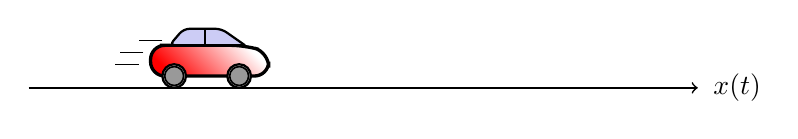
\begin{tikzpicture}
  \begin{scope}[scale=0.3, xscale=-1, xshift=-10cm]
    \shade[top color=red, bottom color=white, shading angle={135}]
    [draw=black,fill=red!20,rounded corners=1.2ex,very thick] (1.5,.5) -- ++(0,1) -- ++(1,0.3) --  ++(3,0) -- ++(1,0) -- ++(0,-1.3) -- (1.5,.5) -- cycle;
    \draw[very thick, rounded corners=0.5ex,fill=black!20!blue!20!white,thick]  (2.5,1.8) -- ++(1,0.7) -- ++(1.6,0) -- ++(0.6,-0.7) -- (2.5,1.8);
    \draw[thick]  (4.2,1.8) -- (4.2,2.5);
    \draw[draw=black,fill=gray!50,thick] (2.75,.5) circle (.5);
    \draw[draw=black,fill=gray!50,thick] (5.5,.5) circle (.5);
    \draw[draw=black,fill=gray!80,semithick] (2.75,.5) circle (.4);
    \draw[draw=black,fill=gray!80,semithick] (5.5,.5) circle (.4);
    \draw[thin, ] (7,1) -- (8,1);
    \draw[thin, ] (6.8,1.5) -- (7.8,1.5);
    \draw[thin, ] (6,2) -- (7,2);
\end{scope}

  
  \draw[->,semithick] (-.5,0) -- (8,0);
  \draw (8.5,0) node {$x(t)$};
\end{tikzpicture}
\end{center}

Un coche va a velocidad constante en una autopista horizontal. En la instante $t=t_1$, el conductor empuje el clutch, desconectando el motor y las ruedas. Cuál de las siguientes graficas describe mejor la velocidad $v(t)=\dot{x}(t)$ del coche?

\begin{center}
   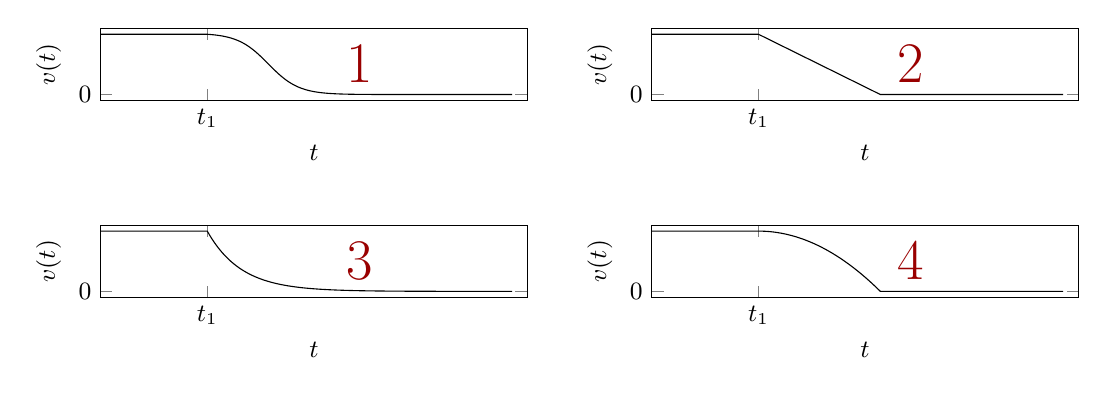
\begin{tikzpicture}
   \small

   \begin{axis}[
   width=7cm,
   height=2.5cm,
   xlabel={$t$},
   ylabel={$v(t)$},
   xmin=-3.5,
   xmax=10.5,
   ytick = {0},
   xtick = {0},
   xticklabels = {$t_1$},
   ]
   \addplot+[black, no marks, domain=-4:10, samples=400,variable=k] { (k < 0) + (k>0)*(1+exp(-4))/(1+exp(4*(0.5*k-1)))};

   \node[black!40!red] at (axis cs: 5, 0.5) {\huge 1};
   \end{axis}

   \begin{axis}[
   xshift=7cm,
   width=7cm,
   height=2.5cm,
   xlabel={$t$},
   ylabel={$v(t)$},
   xmin=-3.5,
   xmax=10.5,
   ytick = {0},
   xtick = {0},
   xticklabels = {$t_1$},
   ]
   \addplot+[black, no marks, domain=-4:10, samples=400,variable=k] { (k<0) + ((k>=0) - (k>4))*(1/4*(4-k)) };
   \node[black!40!red] at (axis cs: 5, 0.5) {\huge 2};
   \end{axis}

   \begin{axis}[
   xshift=0cm,
   yshift=-2.5cm,
   width=7cm,
   height=2.5cm,
   xlabel={$t$},
   ylabel={$v(t)$},
   xmin=-3.5,
   xmax=10.5,
   ytick = {0},
   xtick = {0},
   xticklabels = {$t_1$},
   ]
   \addplot+[black, no marks, domain=-4:10, samples=400,variable=k] { (k<0) + (k>0)*exp(-0.9*k)};
   \node[black!40!red] at (axis cs: 5, 0.5) {\huge 3};
   \end{axis}

   \begin{axis}[
   xshift=7cm,
   yshift=-2.5cm,
   width=7cm,
   height=2.5cm,
   xlabel={$t$},
   ylabel={$v(t)$},
   xmin=-3.5,
   xmax=10.5,
   ytick = {0},
   xtick = {0},
   xticklabels = {$t_1$},
   ]
   \addplot+[black, no marks, domain=-4:10, samples=400,variable=k] { (k<0) + ((k>=0) - (k>4))*(1-1/16*pow(-k,2)) };
   \node[black!40!red] at (axis cs: 5, 0.5) {\huge 4};
   \end{axis}


   \end{tikzpicture}

\end{center}
\end{frame}
\begin{frame}[label={sec:org2a28d69}]{Intuicón para sistemas mecanicas - Simución}

\begin{center}
\begin{tikzpicture}
\tikzstyle{damper}=[thick,decoration={markings,  
  mark connection node=dmp,
  mark=at position 0.5 with 
  {
    \node (dmp) [thick,inner sep=0pt,transform shape,rotate=-90,minimum width=15pt,minimum height=3pt,draw=none] {};
    \draw [thick] ($(dmp.north east)+(2pt,0)$) -- (dmp.south east) -- (dmp.south west) -- ($(dmp.north west)+(2pt,0)$);
    \draw [thick] ($(dmp.north)+(0,-5pt)$) -- ($(dmp.north)+(0,5pt)$);
  }
}, decorate]
\tikzstyle{ground}=[fill,pattern=north east lines,draw=none,minimum width=0.75cm,minimum height=0.3cm]

  \begin{scope}[scale=0.3, xscale=-1, xshift=-10cm]
    \shade[top color=red, bottom color=white, shading angle={135}]
    [draw=black,fill=red!20,rounded corners=1.2ex,very thick] (1.5,.5) -- ++(0,1) -- ++(1,0.3) --  ++(3,0) -- ++(1,0) -- ++(0,-1.3) -- (1.5,.5) -- cycle;
    \draw[very thick, rounded corners=0.5ex,fill=black!20!blue!20!white,thick]  (2.5,1.8) -- ++(1,0.7) -- ++(1.6,0) -- ++(0.6,-0.7) -- (2.5,1.8);
    \draw[thick]  (4.2,1.8) -- (4.2,2.5);
    \draw[draw=black,fill=gray!50,thick] (2.75,.5) circle (.5);
    \draw[draw=black,fill=gray!50,thick] (5.5,.5) circle (.5);
    \draw[draw=black,fill=gray!80,semithick] (2.75,.5) circle (.4);
    \draw[draw=black,fill=gray!80,semithick] (5.5,.5) circle (.4);
    \draw[thin, ] (7,1) -- (8,1);
    \draw[thin, ] (6.8,1.5) -- (7.8,1.5);
    \draw[thin, ] (6,2) -- (7,2);
    \node[coordinate] (fender) at (6.5, 1.5) {};
\end{scope}

  \draw[semithick] (-0.5,0) -- (-0.5, 1);
  \draw[damper] (-0.5, 0.5 |- fender) -- (fender);
  \node[ground, rotate=90, anchor=south] at (-0.5, 0.5) {};
  \draw[->,semithick] (-.5,0) -- (8,0);
  \draw (8.5,0) node {$x(t)$};
\end{tikzpicture}
\end{center}

mass \(m = \unit{1000}{\kilo\gram}\), friction coefficient \(f=\unit{20}{\newton\per(\meter\per\second)}\)
\end{frame}


\begin{frame}[label={sec:org0c3a87c}]{Intuición para sistemas electricas}
\begin{columns}
\begin{column}{0.4\columnwidth}
\begin{center}
\includegraphics[height=0.8\textheight]{../../figures/RC-circuit}
\end{center}

\#+begin\textsubscript{export} latex
\begin{center}
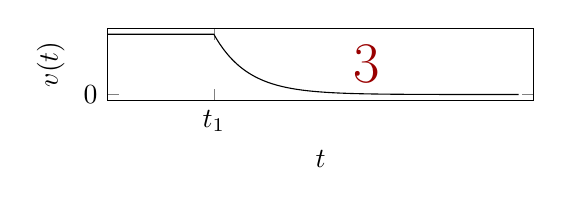
\begin{tikzpicture}
\begin{axis}[
xshift=0cm,
yshift=-2.5cm,
width=7cm,
height=2.5cm,
xlabel={$t$},
ylabel={$v(t)$},
xmin=-3.5,
xmax=10.5,
ytick = {0},
xtick = {0},
xticklabels = {$t_1$},
]
\addplot+[black, no marks, domain=-4:10, samples=400,variable=k] { (k<0) + (k>0)*exp(-0.9*k)};
\node[black!40!red] at (axis cs: 5, 0.5) {\huge 3};
\end{axis}
\end{tikzpicture}
\end{center}
\#+end\textsubscript{export} latex
\end{column}

\begin{column}{0.6\columnwidth}
\alert{Actividad individual} Al principio (\(t=0\)) el circuito está abierto y no hay carga en el capacidor. En el instante \(t=0\) el interruptor S cierre el circuito y lo mantiene cerrado. Grafica el voltage sobre el capacidor como función de tiempo. El constante de tiempo del sistem es \(\tau=RC\), y determine el comportamiento del sistema. Indica en tú gráfica como se puede identificar \(tau\). 

Tomo fotó y mandamelo por \alert{Remind}.
\end{column}
\end{columns}
\end{frame}


\begin{frame}[label={sec:orgb0433e8}]{Intuition for electrical circuits - Simulation}
Let \(R=\unit{1}{\kilo}\Omega\) and \(C = \unit{100}{\micro\farad}\).

\[ \tau = RC = (1\times 10^{3})(100\times 10^{-6}) = \unit{10^{-1}}{\second} \]
\end{frame}
\end{document}